% Manually converted from "Dolphin樂譜編輯器L.doc" on January 20, 2012
%-----------------------------------------------------------------
% Use the following command to compile: xelatex -interaction=nonstopmode dolphin.tex
% Todo:
% * fix figures
% * fix references

\documentclass[12pt,a4paper,oneside]{report}
\usepackage{fontspec} 
\usepackage{xeCJK} 
% \usepackage{mathtools} % can not be found in Ubuntu
\usepackage{amsmath} % for equations
\usepackage{url} % for \url
\usepackage{graphicx} % for images
\usepackage{chngcntr} % for fixing figure numbering, see http://www.tex.ac.uk/cgi-bin/texfaq2html?label=running-nos

%set chinese font
%\setCJKmainfont{AR PL UMing TW} 
\setCJKmainfont{cwTeXFangSong} 
%\setCJKmainfont{cwTeXKai} 
%\setCJKmainfont{cwTeXMing} 

%handle chinese newline
\XeTeXlinebreaklocale "zh"
\XeTeXlinebreakskip = 0pt plus 1pt

%custom abstract title
\renewcommand{\abstractname}{摘要} 

%custom chapter title
%\renewcommand{\chaptername}{章}
%\renewcommand{\chaptername}{第\CJKnumber{\thechapter}章}

%custom content title
\renewcommand{\contentsname}{目錄}

%custom figure title
\renewcommand{\figurename}{圖}

%paragraph spacing
\parskip 7.2pt

%label numbering style
%\renewcommand{\thefigure}{\arabic{figure}}
\counterwithout{figure}{chapter}

% args: label, filename, scale, caption
\newcommand{\figurewithcaption}[4] {
   %[htb] means placing the figure here, at the top, or at the bottom, order means preference, see http://www.sci.utah.edu/~macleod/latex/latex-figures.html
   \begin{figure}[htb]
   \centering
   \includegraphics[scale=#3]{#2}
   \caption{#4}
   \label{#1} % whatch out for any white space inside braces
   \end{figure}
}

\begin{document}

\title{Dolphin 樂譜編輯器}
\date{\today}
\maketitle

%\begin{abstract} % not very useful in Chinese
%\thispagestyle{empty} % suppress page number
\begin{center}
Dolphin 樂譜編輯器

摘要
\end{center}

我們開發出一套所見即所得的樂譜編輯器Dolphin,支援即時五線譜與簡譜的轉換及MIDI檔與樂譜的轉換等進階功能,另外也支援各種輸入方式如MIDI裝置輸入、虛擬鍵盤輸入及哼唱輸入等。Dolphin還具備腳本編輯器讓使用者撰寫腳本來控制樂譜。我們相信這些自動化的功能可大幅改善樂譜編輯器的可用性並使其用途更為廣泛。

關鍵詞:樂譜編輯器、音樂函式庫、自動旋律轉錄

%\end{abstract}

\tableofcontents

\chapter{緒論}
\section{研究背景與動機}
% \addtocontents{toc}{}
% Why did you want to do it? What was your goal? 

樂譜編輯器(musical notation editor, scorewriter)是用來輸入、編輯及輸出樂譜或音樂的軟體;其之於樂譜的關係就如同文書處理器(word processor)之於文書。相較於傳統的方式,樂譜編輯器可利用各種自動化的工具簡化並加速樂譜的處理流程,且產生出的樂譜較手寫更為美觀,方便用來出版、散佈,作為教學、觀摩或演奏之用。

除了產生樂譜之外,多數樂譜編輯器也可將編輯中的樂譜播放出來,功能類似音訊器(Sequencer)>>>;然而,音訊器主要用來錄製及播放音樂,而樂譜編輯器的播放功能主要用來輔助編輯樂譜。樂譜編輯器也可產生音訊檔,該檔案可直接用來交流、分享,也可交由數位音訊軟體做進一步的混音和後製。

市面上的樂譜編輯器多以五線譜來呈現。然而除了五線譜外,世界各地仍流行多種記錄音樂的系統,簡潔易讀的簡譜(numbered musical notation)便是其中之一。簡譜屬於文字譜的一種\cite{chinaEncyclopedia},是以阿拉伯數字「1234567」記寫音階階名的譜式\footnote{在此採《中國音樂史.樂譜篇》中「數字簡譜」\cite{chinaMusicHistory}的定義。}。簡譜的歷史悠久。中國唐朝(618–907)出現的工尺譜便含有簡譜的影子,其所使用的「上、尺、工、凡、六、五、乙」可對應至簡譜的一至七\cite{wiki};在十六世紀的中東,有以波斯數字記寫音階的記譜法;而後在十七至十九世紀的歐洲則有盧梭等人的改良及推廣。日本、爪哇島及峇里島亦存有類似的系統\cite{britannica}。簡譜在清朝由日本傳入中國,當時便廣為新式學堂所用。今日簡譜仍經常用於音樂教學,以及坊間的流行歌本中。

鋼琴捲譜(piano roll notation)是另一種樂譜編輯器常缺乏的記譜法。鋼琴捲譜屬於圖像譜的一種,因形似鋼琴捲(piano roll)而得名。鋼琴捲是一種早期的音樂儲存媒介,藉由在紙捲上打孔來記錄音符的資訊,由以氣壓驅動的自奏鋼琴(player piano)讀取並將樂曲彈奏出來。鋼琴捲在一九二零年代曾相當流行,而後逐漸被收音機和唱片所取代\cite{thePiano}。今日的鋼琴捲譜多以橫軸代表時間,縱軸代表音高,譜中長短不一的矩形則代表音符,矩形的長短決定音符的時值;這樣的表示方式相當直覺,初學者也易於上手。

%[htb] means placing the figure here, at the top, or at the bottom, order means preference, see http://www.sci.utah.edu/~macleod/latex/latex-figures.html
\begin{figure}[htb]
\centering
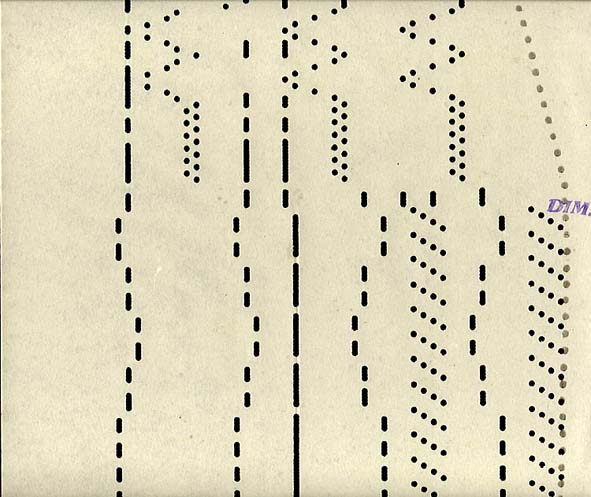
\includegraphics[scale=0.3]{img/piano_roll.png}
\caption{ 早期的鋼琴捲(圖片來源:http://website.lineone.net/~agr/rollscan2.html) }
\label{fig:piano_roll} % whatch out for any white space inside braces
\end{figure}


在輸入方面,大部分的樂譜編輯器支援滑鼠輸入,可以點擊或拖拉的方式來新增、修改音符。也有部分支援鍵盤輸入,透過按鍵對應,或以組合鍵的方式來輸入音符,操作方式如同作業系統的輸入法(input method)。雖然相較於紙筆,這類方式已簡便許多,但對不熟悉樂理的初學者或演奏者而言,輸入樂譜仍往往是件困難的工作。

此外,目前的樂譜編輯器也普遍不支援腳本(script)功能。在Word中使用者可以VBScript來操控文件,而Photoshop則支援以JavaScript來處理圖像。若能以腳本來控制樂譜,使用者便可發揮創意,自行撰寫腳本來擴充樂譜編輯器的功能,例如應用在電腦產生音樂(computer-generated music)或音樂分析(musical analysis)等領域上。

因此,我們開發出一套樂譜編輯器Dolphin,能以五線譜、簡譜和鋼琴捲譜來呈現樂譜,並支援多種自動化的功能來輔助使用者輸入,例如能將現有的音樂檔案自動轉換為樂譜,以演奏的方式輸入樂譜,甚至直接將使用者的哼唱轉換為樂譜。Dolphin也能讓使用者撰寫腳本來擴充或自創特殊的功能。

\section{相關研究}

Sibelius[]是一套熱門的樂譜編輯器。除了具有編輯、排版及輸出樂譜的功能之外,也包含許多進階的功能。如Flexi-time可即時地將MIDI鍵盤的彈奏轉錄為樂譜。PhotoScore則可將印刷樂譜掃描至編輯器。Scorch瀏覽器外掛可讓未安裝Sibelius的一般使用者透過瀏覽器線上觀看樂譜。然而,Sibelius並未提供腳本功能,也無法以麥克風來輸入樂譜。

Finale[]是另一套知名的樂譜編輯器,被視為Sibelius的主要競爭者。如同Sibelius,Finale中的SmartScore也可掃描樂譜,而其MicNotator不僅可辨認MIDI裝置,也能透過麥克風將銅管或木管樂器的彈奏轉錄為樂譜。FinaleScript為Finale專屬的腳本語言,使用者可利用該語言撰寫腳本。不過Finale的MicNotator並不適用於人聲,且其只能使用單一語言來撰寫腳本。

Denemo[]是一套開放原始碼的樂譜編輯器,可視為LilyPond[]的GUI介面。除了可使用鍵盤、滑鼠輸入音符之外,也可以MIDI裝置或以麥克風接收樂器的聲音來輸入。不過如同Finale,其麥克風的輸入仍不適用於人聲。

Music MasterWorks[]是一套特殊的樂譜編輯器,其voice-to-note功能可將人的哼唱轉為樂譜,內含的singing analysis還可用來分析哼唱者的音準表現。但其voice-to-note得在錄音結束後才能看到樂譜,無法即時地對使用者的哼唱產生適當的回饋。

哼唱鈴i-Ring[]是一套可用哼唱方式製作手機鈴聲的音樂工具。然而如同Music MasterWorks,必須在錄音結束後才能看到轉換結果,三十秒的錄音時限及只適合接收「他-他-他」的音也限縮了不少自由度。

\section{論文大綱}

在下一章我們介紹Dolphin 所使用到的基礎程式庫。第三章介紹Dolphin及其主要特色。第四章介紹編輯器的設計及實作,最末章為結論及展望。//>>>

\chapter{Dolphin概觀}
% What did you do? What is Dolphin? What can I do with it?

Dolphin是一個所見即所得的樂譜編輯器,具備完整的功能輔助使用者編輯樂譜。圖~\ref{fig:screenshot}為系統的截圖。

\begin{figure}[htb]
\centering
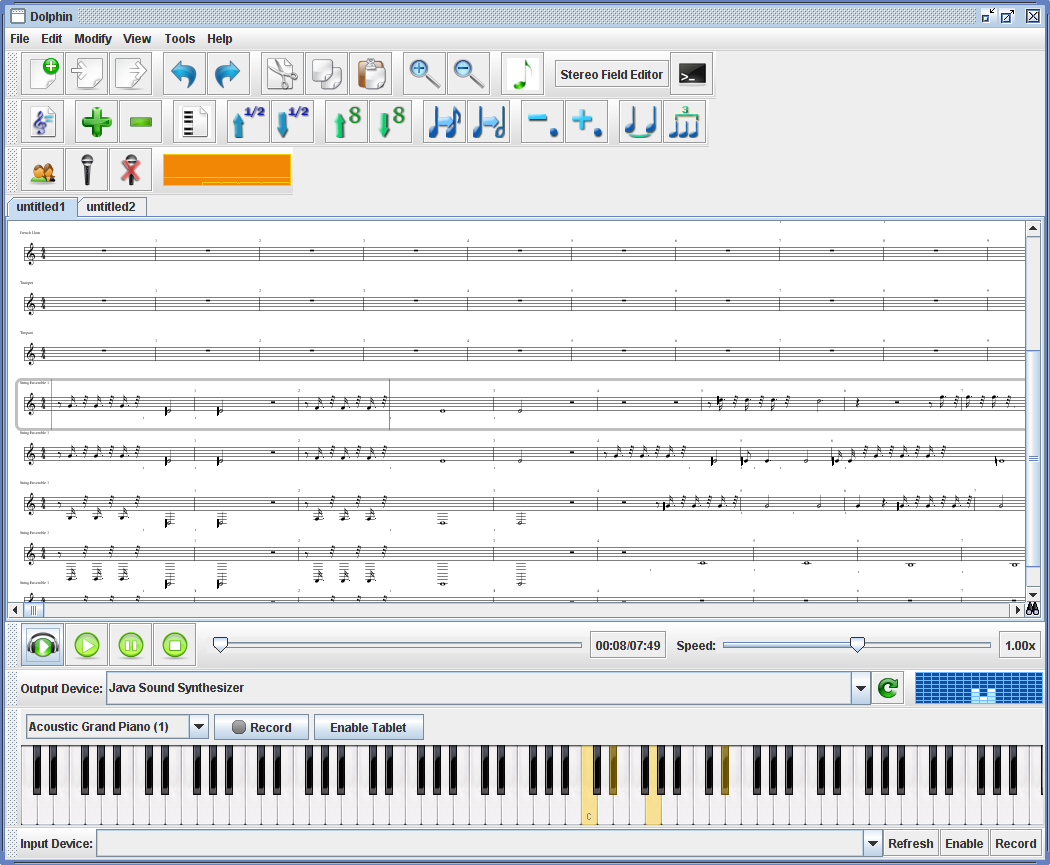
\includegraphics[scale=0.3]{img/screenshot.png}
\caption{ Dolphin執行畫面}
\label{fig:screenshot}
\end{figure}

Dolphin可讓使用者選擇匯入MIDI檔編輯,或自行創作新的樂譜。樂譜的各聲部可獨立以五線譜、簡譜或鋼琴捲譜來檢視,也可任意調整縮放。使用者可編輯樂譜的各項屬性,並為樂譜新增聲部和音符。在輸入時,可選擇以滑鼠在譜上點擊或用鍵盤以類似輸入法的方式來輸入音符,也可以彈奏畫面上的虛擬MIDI鍵盤或外接的實體MIDI鍵盤來輸入。使用者也可以直接對著麥克風哼唱來輸入,Dolphin會自動將哼唱轉換為對應的音符。Dolphin支援無次數限制的復原和重做,使用者不必擔心輸入錯誤。在編輯過程中也可以隨時播放樂譜,也可開啟立體聲編輯器在播放過程中即時地編輯立體聲的效果。若使用者會撰寫程式,也可開啟腳本編輯器,以JavaScript、Python或Ruby等語言撰寫腳本來控制或分析樂譜。

Dolphin的主要特色列舉如下:
\begin{enumerate}
\item 五線譜、簡譜及鋼琴捲譜的編修。
      各聲部皆可獨立調整以五線譜、簡譜或鋼琴捲譜來顯示、編輯。
\item 匯入、匯出MIDI 檔。
      可匯入現有的MIDI檔,也可將樂譜匯出為MIDI檔。
\item 樂譜播放。
      可播放編輯中的樂譜,調整播放進度和速度,也可調整輸出的MIDI裝置。
\item 立體聲編輯器。
      透過平面圖編輯各聲部樂器的位置以模擬立體聲的效果。
\item 腳本編輯器。
      可以JavaScript、Python、Ruby等多種語言撰寫腳本(script)來控制編輯器或樂譜。
\item 復原、重做。
      支援無次數限制的復原和重做。
\item 樂譜縮放。
      樂譜檢視可任意放大、縮小。
\item 多檔編輯、單檔多窗。
      可同時編輯多個檔案,單檔也可以顯示於多個編輯窗,各編輯窗皆可編輯並會同步更新。
\item 哼唱輸入。
      支援以哼唱方式來輸入音符。
\item 虛擬MIDI鍵盤輸入。
      可彈奏螢幕上的虛擬MIDI鍵盤來輸入音符。
\item MIDI裝置輸入。
      可彈奏實體MIDI裝置如MIDI鍵盤來輸入音符。 
\end{enumerate}

\chapter{使用說明書}
% how to use it?
\section{操作環境}
\subsection{主視窗}
\subsection{工具列}
/* 
解說視窗各區域
*/

/* 
解說menu bar及其使用
*/
\section{編輯樂譜}
   \subsection{空白樂譜}
   \subsection{由MIDI 檔匯入}
\section{編輯聲部}
   \subsection{修改聲部屬性}
   \subsection{選擇譜式}
\section{編輯音符}
   \subsection{滑鼠輸入}
   \subsection{鍵盤輸入}
   \subsection{虛擬鍵盤輸入}
   \subsection{MIDI 鍵盤輸入}
   \subsection{哼唱輸入}
   \subsection{修改音符}
\section{匯出MIDI 檔}
\section{樂譜播放器}
\section{腳本編輯器}
\section{立體聲編輯器}

\chapter{設計與實作} 
% How did you implement it?

\section{系統架構}


\begin{figure}[htb]
\centering
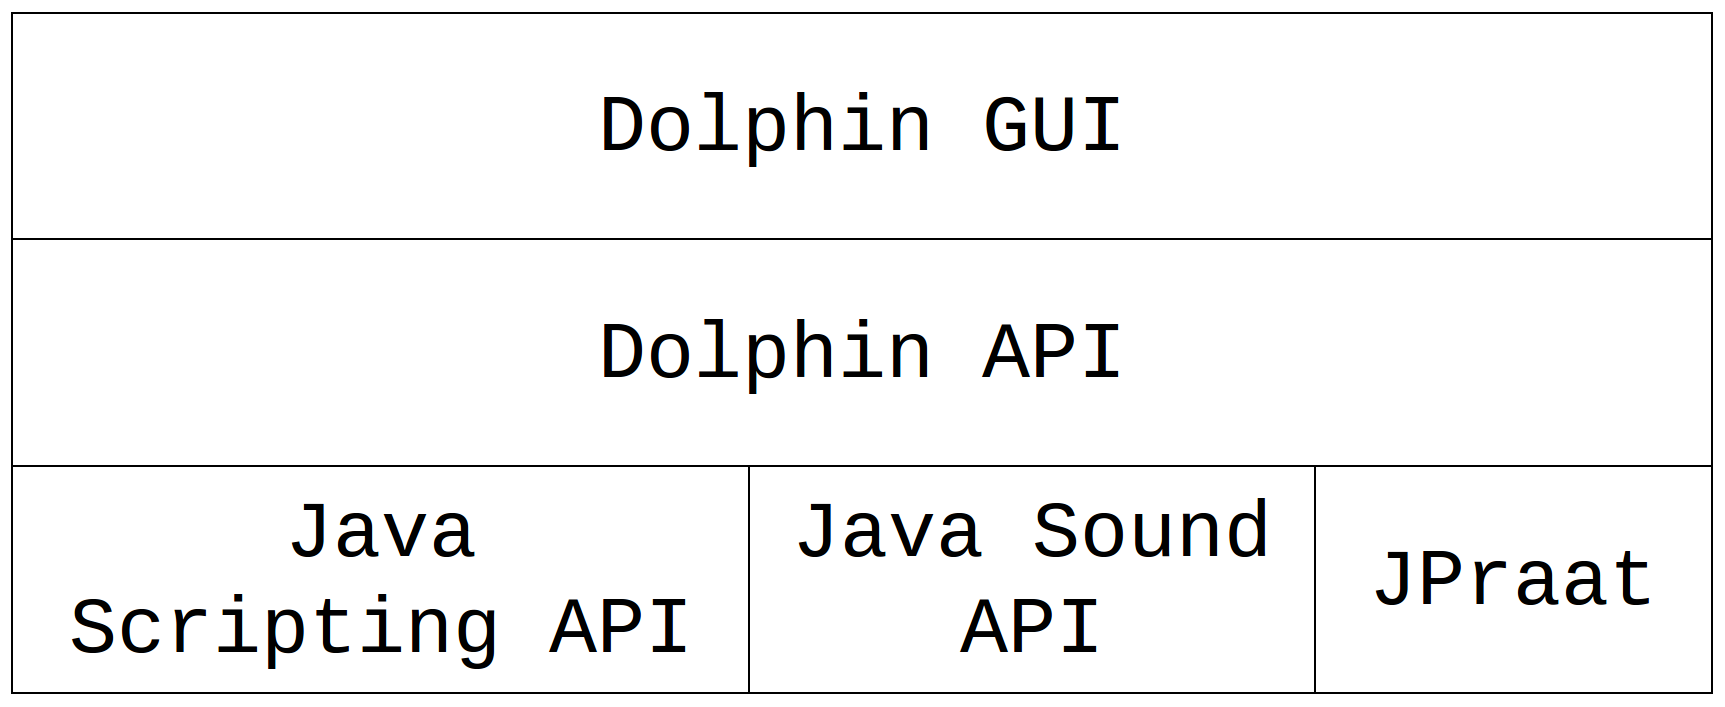
\includegraphics[scale=0.2]{img/framework.png}
\caption{ Dolphin架構圖}
\label{fig:framework}
\end{figure}

圖\ref{fig:framework}為本系統的架構圖。Dolphin以Java語言實作,主要可分為Dolphin API和Dolphin GUI兩個部分。Dolphin API為系統的核心,包含樂譜模型、演算法及訊息傳遞機制,為一套獨立且可重複使用的音樂函式庫。Dolphin GUI為系統的圖形使用者介面,包含用來顯示和編輯樂譜的編輯窗以及各式面板和工具列。

在底層方面,我們使用JPraat來處理哼唱輸入的聲音樣本。使用Java Sound API來處理聲音的擷取以及與MIDI相關的各項功能,如樂譜的播放及MIDI裝置的輸入等。Java Scripting API則用來實作腳本編輯器。


/* 
解說 Dolphin API 含有哪些主要類別, 各含哪些主要方法
*/

/* 
解說 Dolphin GUI 含有哪些主要類別, 各含哪些主要方法
*/

\section{基礎程式庫}
% What third-party librares did you use?

本章介紹Dolphin所用到的函式庫,包含Java Sound API[]的MIDI子套件、Java Scripting API[]及JPraat。其中,Java Sound API和Java Scripting API已內建於Java SE[]中,而JPraat則包含於Dolphin中,使用者皆不需再安裝額外的函式庫。

\subsection{Java Sound API MIDI子套件}

Java SE 含有一套可處理聲音的低階函式庫Java Sound API,可處理採樣和MIDI兩種類型的聲音,本節介紹其MIDI子套件。

\begin{figure}[htb]
\centering
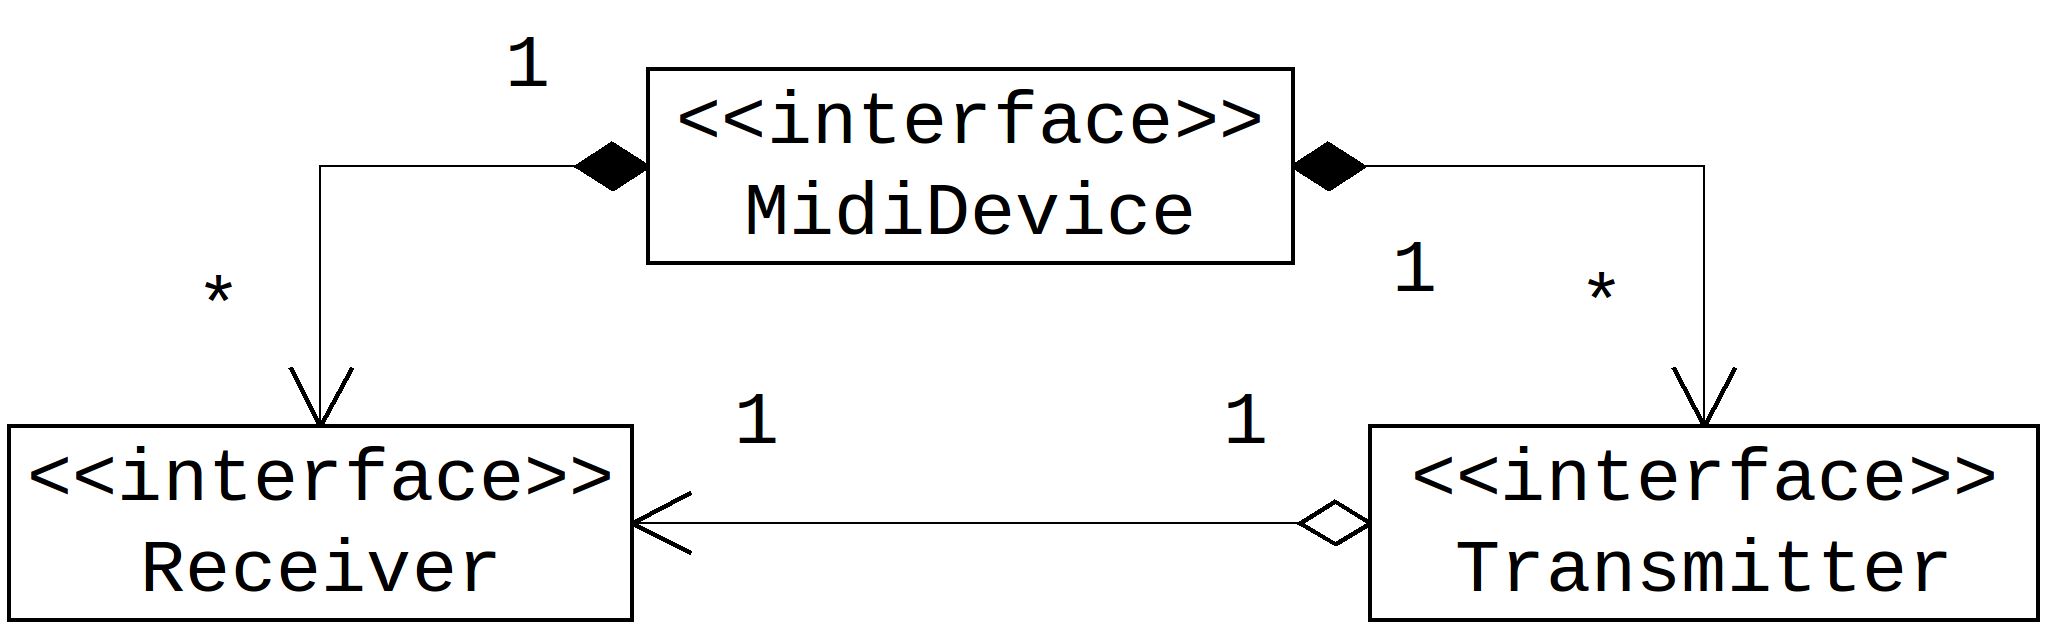
\includegraphics[scale=0.15]{img/mididevice.png}
\caption{ MidiDevice的類別圖 }
\label{fig:mididevice}
\end{figure}

MIDI子套件可分為Wire Protocol和MIDI檔兩大部分。Wire Protocol代表動態的MIDI系統,其主要類別為MidiDevice。MidiDevice含有Transmitter和Receiver,如圖~\ref{fig:mididevice}所示,Transmitter如同MidiDevice的輸出端,而Receiver則如同MidiDevice的輸入端;各MidiDevice以Transmitter和Receiver互相連接。有些MidiDevice會產生MidiEvent(如MIDI鍵盤),有些MidiDevice會接收MidiEvent(如合成器)。在此系統中,MidiDevice會互相合作以達成工作。

/*
     解說你有用到的主要類別, 並各自解說你有用到的主要方法
*/




Sequence則用來模擬靜態的MIDI檔。圖~\ref{fig:sequence}為Sequence所定義的資料結構。其中,Sequence代表整首樂曲,其內含有零至多個Track,Track代表音軌,含有零至多個MidiEvent, MidiEvent表示MIDI事件,含有時間戳記,用來記錄事件的發生時間,及一個MidiMessage,用來記錄事件的內容。我們可將Sequence視為MidiEvent的集合。

\begin{figure}[htb]
\centering
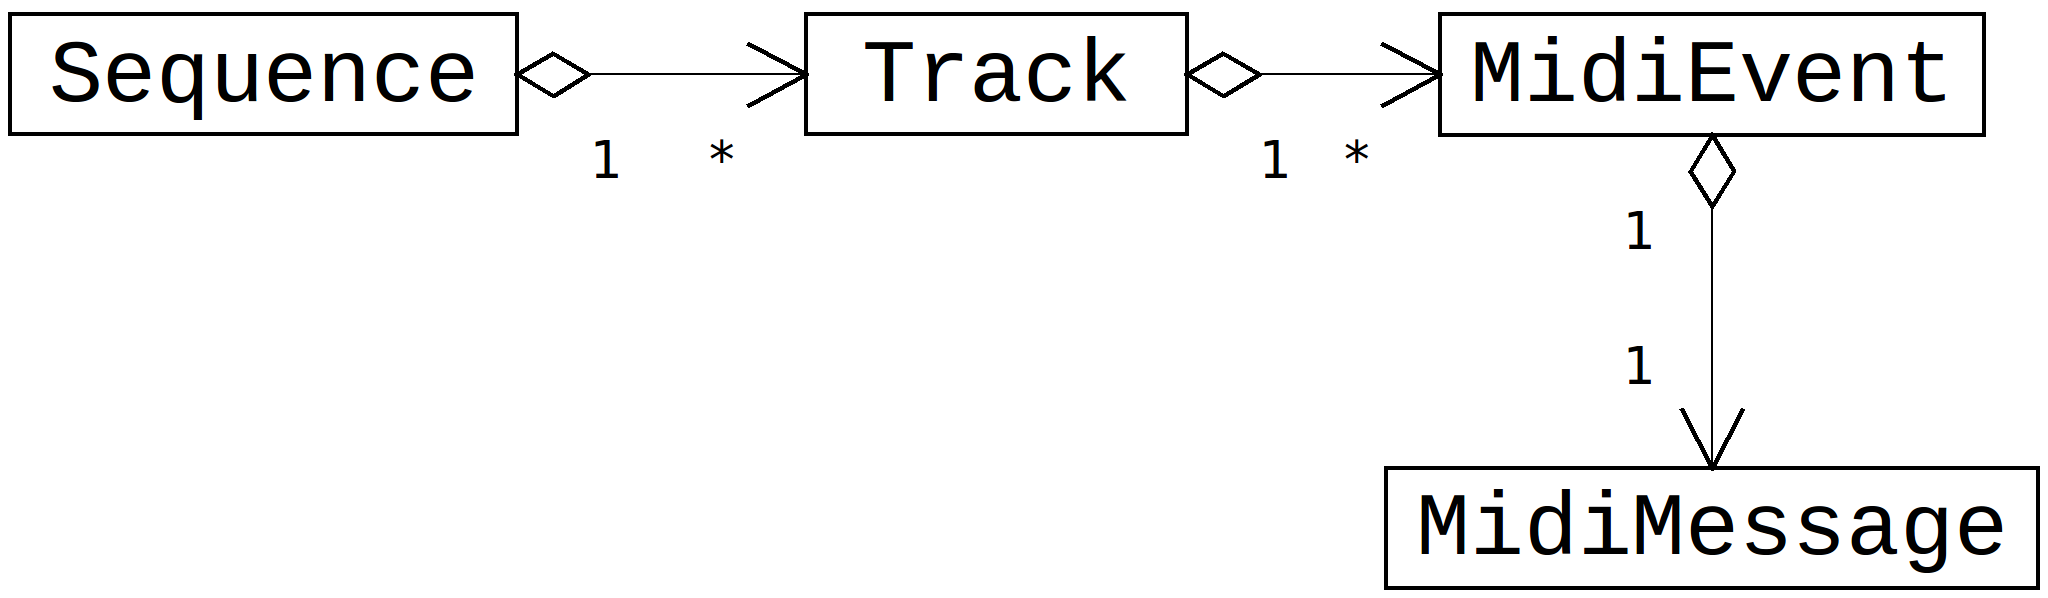
\includegraphics[scale=0.15]{img/sequence.png}
\caption{ Sequence 的類別圖 }
\label{fig:sequence}
\end{figure}

MidiEvent的時間戳記以樂曲開頭為起點,隨著時間遞增,其單位由Sequence的divisionType和resolution來決定。divisionType主要可分為PPQ(purses/ticks per quarter note)和SMPTE (ticks per frame)兩種,而SMPTE還可依FPS(frames per second)值分為24、25、29.97和30四種;resolution則通常為2的倍數,如120、240、480等,越高越精確。當divisionType為PPQ時,resolution的值代表每個四分音符含有的時間戳記;當divisionType為SMPTE時,resolution則代表每個frame含有的時間戳記。

MidiMessage由一串位元組所組成,其中,最常見的是以0x9開頭的Note On訊息和以0x8開頭的Note Off訊息,分別用來模擬樂器聲音的「放」和「收」,例如鋼琴的鍵落和鍵起。一個Note On訊息和其後的一個Note Off訊息合起來便可形成一個音。

/*
     解說你有用到的主要類別, 並各自解說你有用到的主要方法
*/

\subsection{Java Scripting API}

Java Scripting API位於javax.script中,是一個獨立於腳本語言(scripting language)的直譯器使用介面。目前Java SE內建有JavaScript的直譯器,在Java Scripting API的專案頁上也提供如Python、Ruby、AWK等二十幾種語言的直譯器讓使用者自行下載、擴充。

Java SE中的JavaScript直譯器具有LiveConnect功能,可在JavaScript中匯入Java的類別和套件來使用,另外如Ruby的直譯器JRuby、Python的直譯器Jython等多種直譯器也提供了類似的溝通機制。而Java Scripting API也提供綁定(bindings)的機制讓直譯器在執行期直接使用底層Java虛擬機器所含物件的公開介面,我們利用該功能讓腳本編輯器得以操作Dolphin及其內的樂譜。

/*
     解說你有用到的主要類別, 並各自解說你有用到的主要方法
*/


\section{樂譜模型}

Java Sound API中的Sequence是MIDI檔的模型,Sequence僅記錄MIDI訊息而不是音符,並不適合所見即所得的樂譜編輯器。因此,我們為Dolphin定義了一套較高階的模型,如圖\ref{fig:model}所示。 /* paragraph是我說的. 要查明它的正式術語! */



\begin{figure}[htb]
\centering
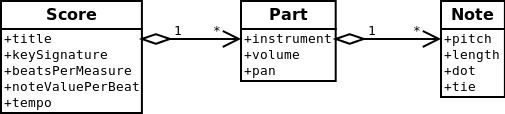
\includegraphics[scale=0.1]{img/model.png}
\caption{ Dolphin的樂譜模型}
\label{fig:model}
\end{figure}

其中,Score代表整首樂譜,具有標題,其內含有零至多個Paragraph,Paragraph代表節/* ? */,含有調號(key signature)、拍號(time signature)及節奏(tempo),節內含有零至多個Part。

/* 各種反覆記號  */ 

Part表示聲部,具有樂器( ? )、音量(volume)及平衡(pan)等屬性,其內包含零至多個Note。Note為音符,含有音高(pitch)、時值(time value)和附點(dot)等資訊。Score便相當對應於Java Sound API中的Sequence,Part則相當對應於Track,而Note則相當對應於MidiEvent。相較於Sequence,Score的模型較易操作,且可以更自然的方式來表示樂譜才合乎人類對樂譜的概念。

樂譜模型的各個類別皆具有存取其屬性的存取函式,而除了音符之外,各類別皆具有
新增、刪除等用來操作模型結構的方法。 /*  
仔細說明  
*/

樂譜還具有復原(undo)、重做(redo),以及通知改動的機制,我們將在討論該機制的運作方式。


\section{樂譜介面}


\begin{figure}[htb]
\centering
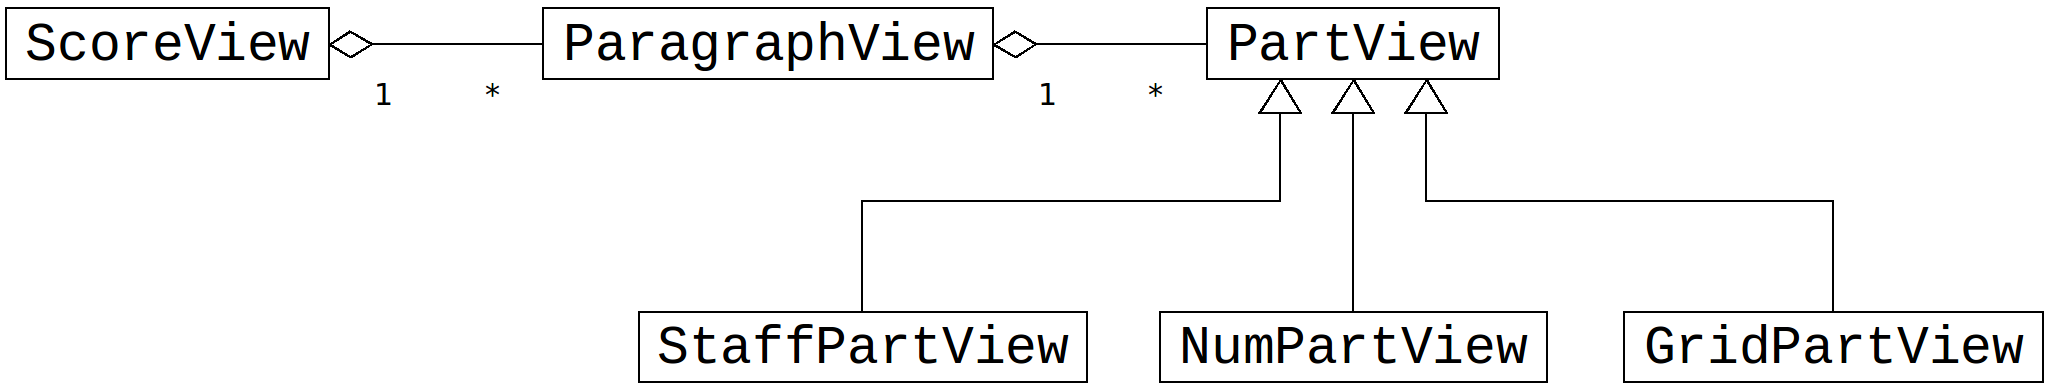
\includegraphics[scale=0.1]{img/view.png}
\caption{ 樂譜介面的類別圖 }
\label{fig:view}
\end{figure}

樂譜介面(ScoreView)負責顯示和操作樂譜(Score),內含對應至節的節介面(ParagraphView)以及對應至聲部(Part)的聲部介面(PartView),如圖~\ref{fig:view} 所示。為了讓各聲部皆可獨立以五線譜、簡譜或是鋼琴捲譜來呈現,我們為聲部介面設計了對應的子類別,包含以五線譜呈現聲部的五線譜聲部介面(StaffPartView),以簡譜來呈現聲部的簡譜聲部介面(NumPartView),以及以鋼琴捲譜來呈現聲部的鋼琴捲譜聲部介面(GridPartView)。三種譜的顯示可在執行期自由切換且不會改動到樂譜。

\begin{figure}[htb]
\centering
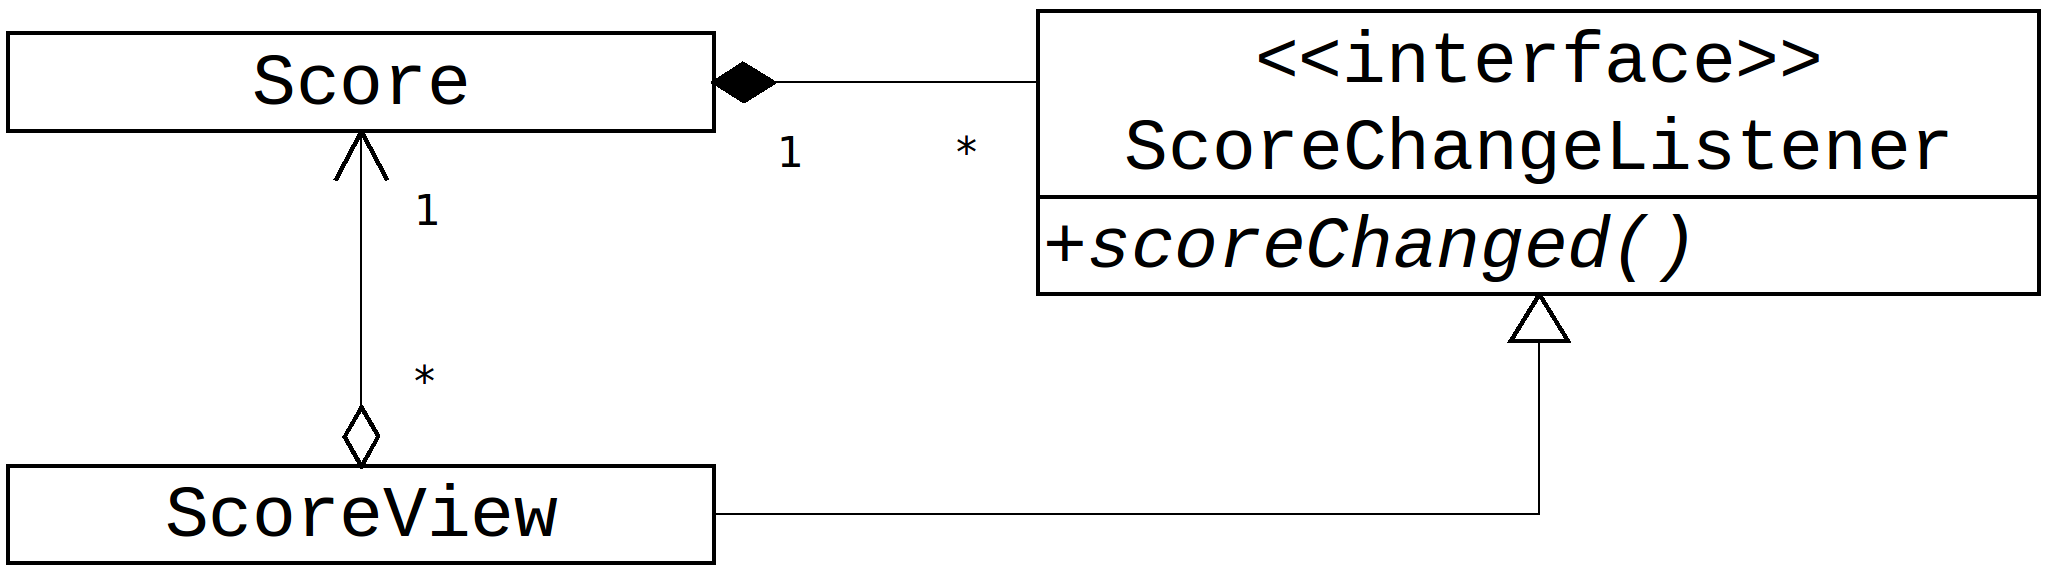
\includegraphics[scale=0.1]{img/model_view.png}
\caption{ 樂譜介面和樂譜模型的連接方式 }
\label{fig:model_view}
\end{figure}

多個樂譜介面可連接至同一個樂譜,然而樂譜並不直接連結至樂譜介面,而是透過樂譜改動傾聽者(ScoreChangeListener)的scoreChanged()方法來與樂譜介面溝通,如圖~\ref{fig:model_view}所示。此設計基於觀察者模式(observer pattern)\cite{designPattern},樂譜並不依賴樂譜介面,可以獨立存在。

樂譜介面同時具有樂譜的操控者和樂譜改動的傾聽者雙重身分。樂譜介面可呼叫公開方法(public method)直接操作樂譜;為確保各傾聽者都能掌握樂譜的最新狀況,當樂譜發生改動時,樂譜會將該其「轉化」為訊息物件,並以此物件通知所有連接到該樂譜的樂譜改動傾聽者,各傾聽者再各自做對應的反應。樂譜並不需要知道各傾聽者在接收到訊息後要做什麼樣的動作,而對樂譜介面而言,此設計也可分離「溝通」和「反應」的程式碼。傳遞的「訊息物件」即為一樂譜改動的實體(instance)。

\subsection{五線譜}
\subsection{簡譜}
\subsection{鋼琴捲譜}
/****
漏講其它各種view
****/

\section{樂譜改動}

\begin{figure}[htb]
\centering
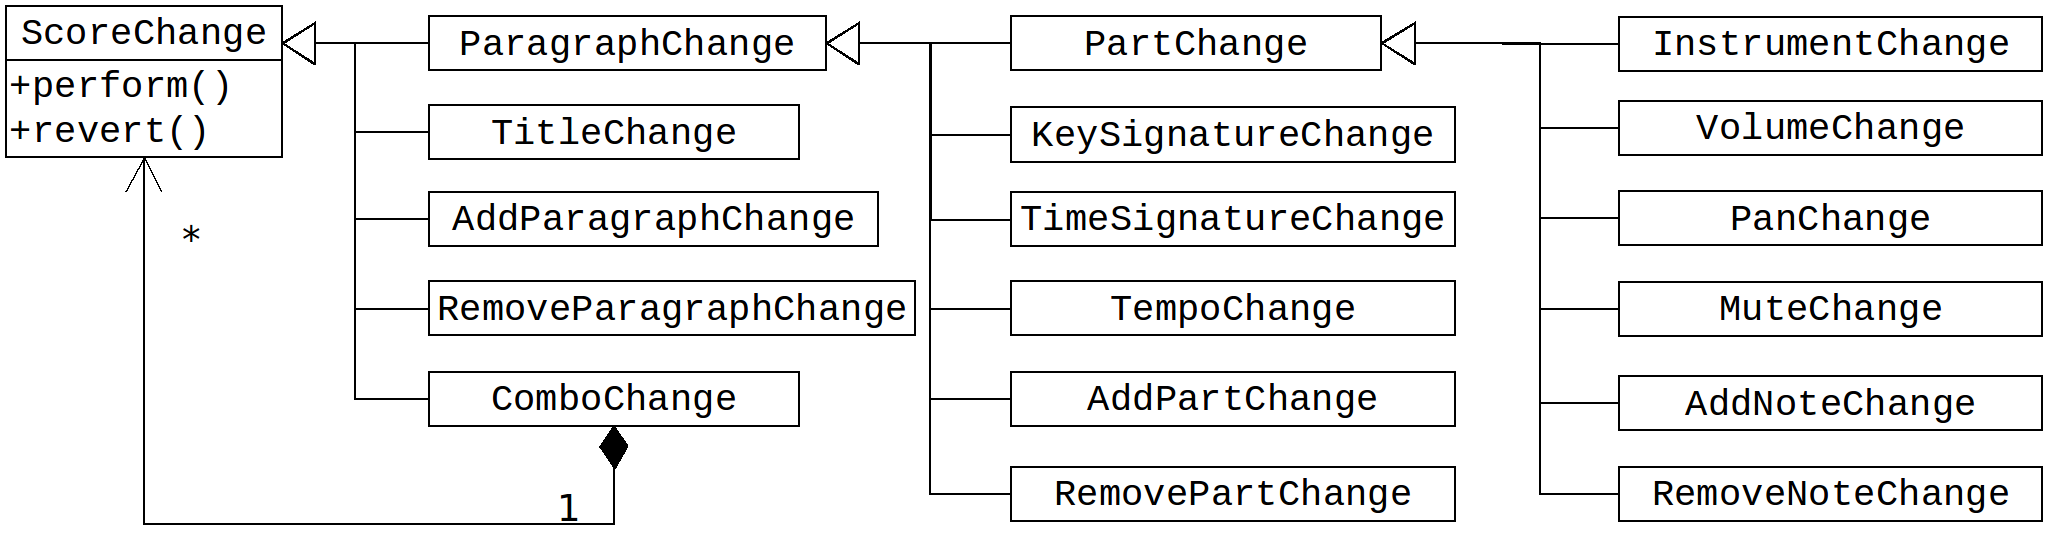
\includegraphics[scale=0.1]{img/changes.png}
\caption{ 樂譜改動的類別圖 }
\label{fig:changes}
\end{figure}


除了後端的模型和前端的介面外,我們也為樂譜(Score)設計了各種樂譜改動(改動,ScoreChange),用來描述樂譜的修改動作並讓樂譜傳遞改動訊息。圖 \ref{fig:changes}為樂譜改動的類別圖,在Dolphin中,樂譜改動的基底類別(base class)為ScoreChange。各種樂譜改動記錄了不同的修改資訊,本身可被執行(perform)和回復(revert),也可以被傳遞、配發給感興趣的傾聽者

樂譜改動有五個子類別,分別為用來描述節內的修改的節改動(ParagraphChange)、描述標題修改的標題改動(TitleChange)、描述新增節的新增節改動(AddParagraphChange)、刪除節的刪除節改動(RemoveParagraphChange)和複合改動(ComboChange)。

複合改動(ComboChange)用來代表多重的改動。複合改動內含一個樂譜改動串列,其本身也是一個樂譜改動。複合改動的「執行」即為依序「執行」其包含的所有改動,而其「復原」即為倒序「復原」串列中的改動,此設計衍生自複合模式(composite pattern)[]。複合改動可讓客戶在執行期自行組裝各種較複雜的動作,例如一個「刪除多個音符」的動作即可拆解為多個基本的刪除音符改動(RemoveNoteChange),而一個「改變音符」的動作則可拆解為一個刪除音符改動和一個新增音符改動(AddNoteChange)。複合改動也可包含其他的複合改動來組成樹狀結構以支援更複雜的動作,例如一個「取代多個音符為一個新音符」的動作即可以一個「刪除多個音符」的複合改動和一個新增音符改動所構成。

節改動有六個子類別,分別為修改聲部的聲部改動(PartChange)、修改調號的調號改動(KeySignatureChange)、修改拍號的拍號改動(TimeSignatureChange)、修改節拍的節拍改動(TempoChange)、新增聲部的新增聲部改動(AddPartChange),以及刪除聲部的刪除聲部改動(RemovePartChange)。

聲部改動也有六個子類別,分別為修改樂器的樂器改動(InstrumentChange)、修改音量的音量改動(VolumeChange)、修改平衡的平衡改動(PanChange)、修改是否靜音的靜音改動(MuteChange)以及新增和刪除音符的新增音符改動(AddNoteChange)和刪除音符改動(RemoveNoteChange)。

樂譜改動有三種不同的狀態。當改動剛被生成時,會處在未執行狀態(unperformed);而當其perform()被呼叫後,會先儲存必要的資訊再執行編輯動作,執行完便進到已執行狀態(performed);再呼叫revert()即會根據儲存的資訊回復先前執行的編輯動作,然後進到已回復狀態(reverted)。已回復的改動可再被執行,再執行後也可再回復。

由於各樂譜改動皆可被執行和回復,我們便可以樂譜改動來實作樂譜的復原(undo)及重做(redo)功能。藉由將改動儲存起來,樂譜能復原已執行的改動,讓樂譜回復至改動發生之前的狀態。例如當樂譜的狀態為S1時,如圖~\ref{fig:undo_redo}所示,樂譜已依序發生了e1、e2和e3三個改動,三個改動皆處在改動串列中,且皆已被執行。此時若執行復原動作,Score會呼叫e3的revert(),然後將next左移一格,代表e3進到已回復狀態,使樂譜狀態成為S2。

/*  
解釋這些ScoreChange 有何方法? 如何使用?   
*/ 


\begin{figure}[htb]
\centering
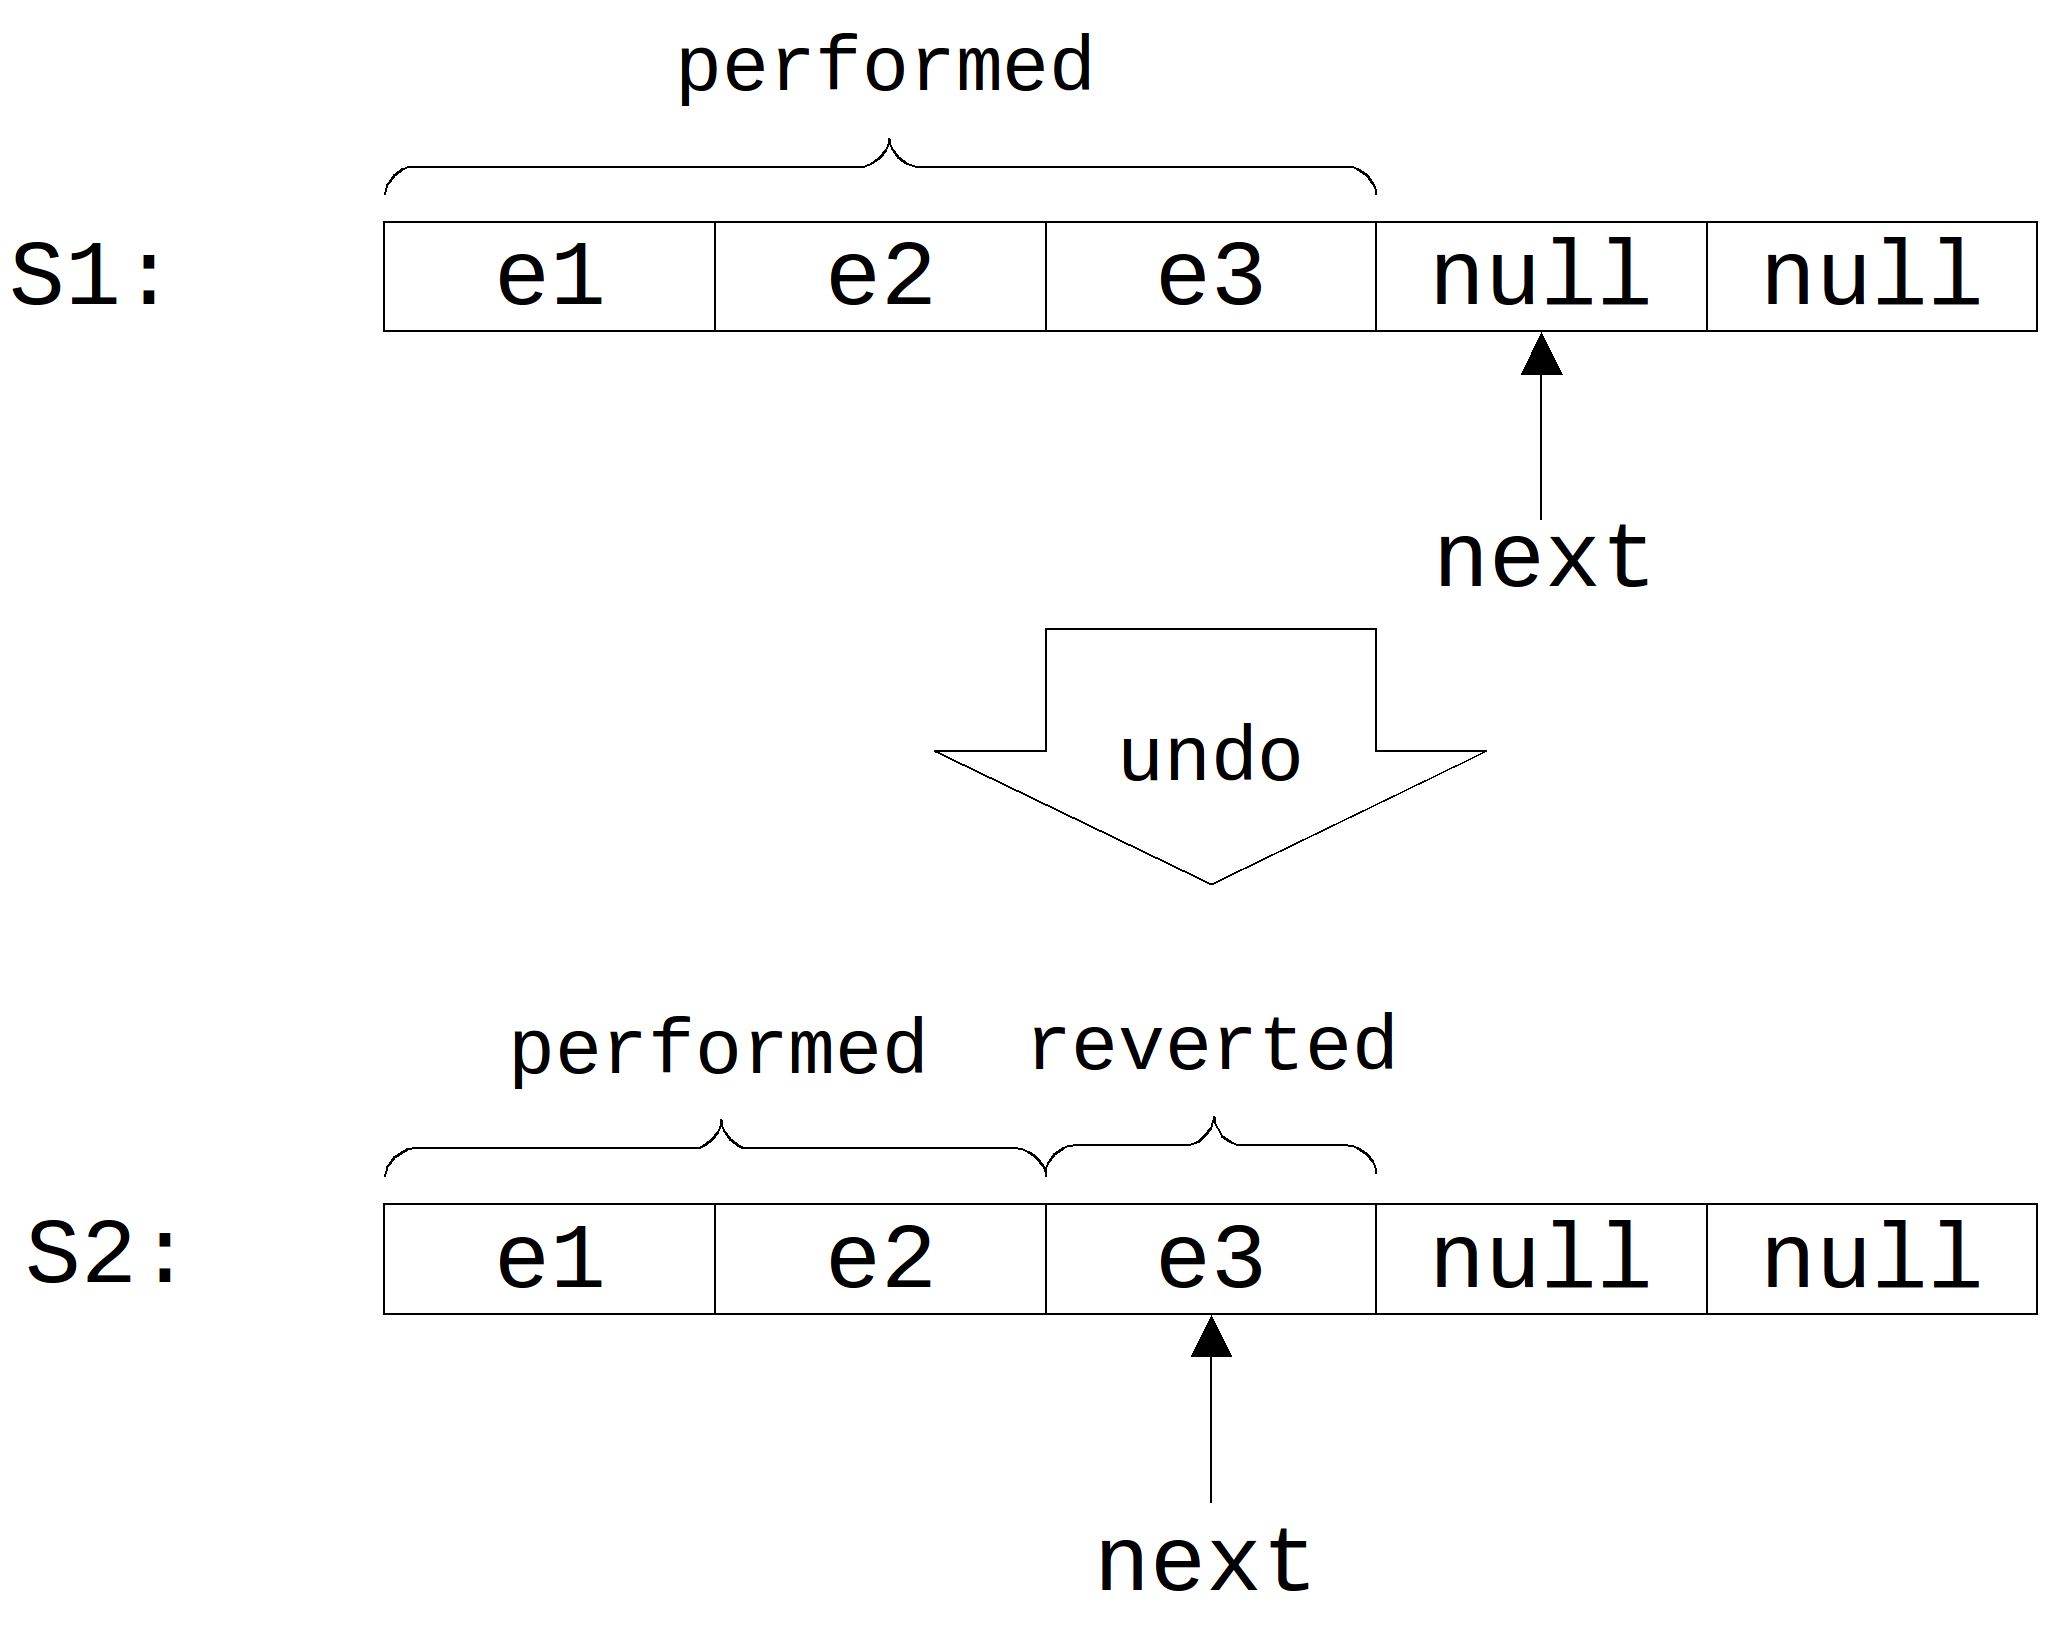
\includegraphics[scale=0.1]{img/undo_redo.png}
\caption{ 復原及重做的運作 }
\label{fig:undo_redo}
\end{figure}

\begin{figure}[htb]
\centering
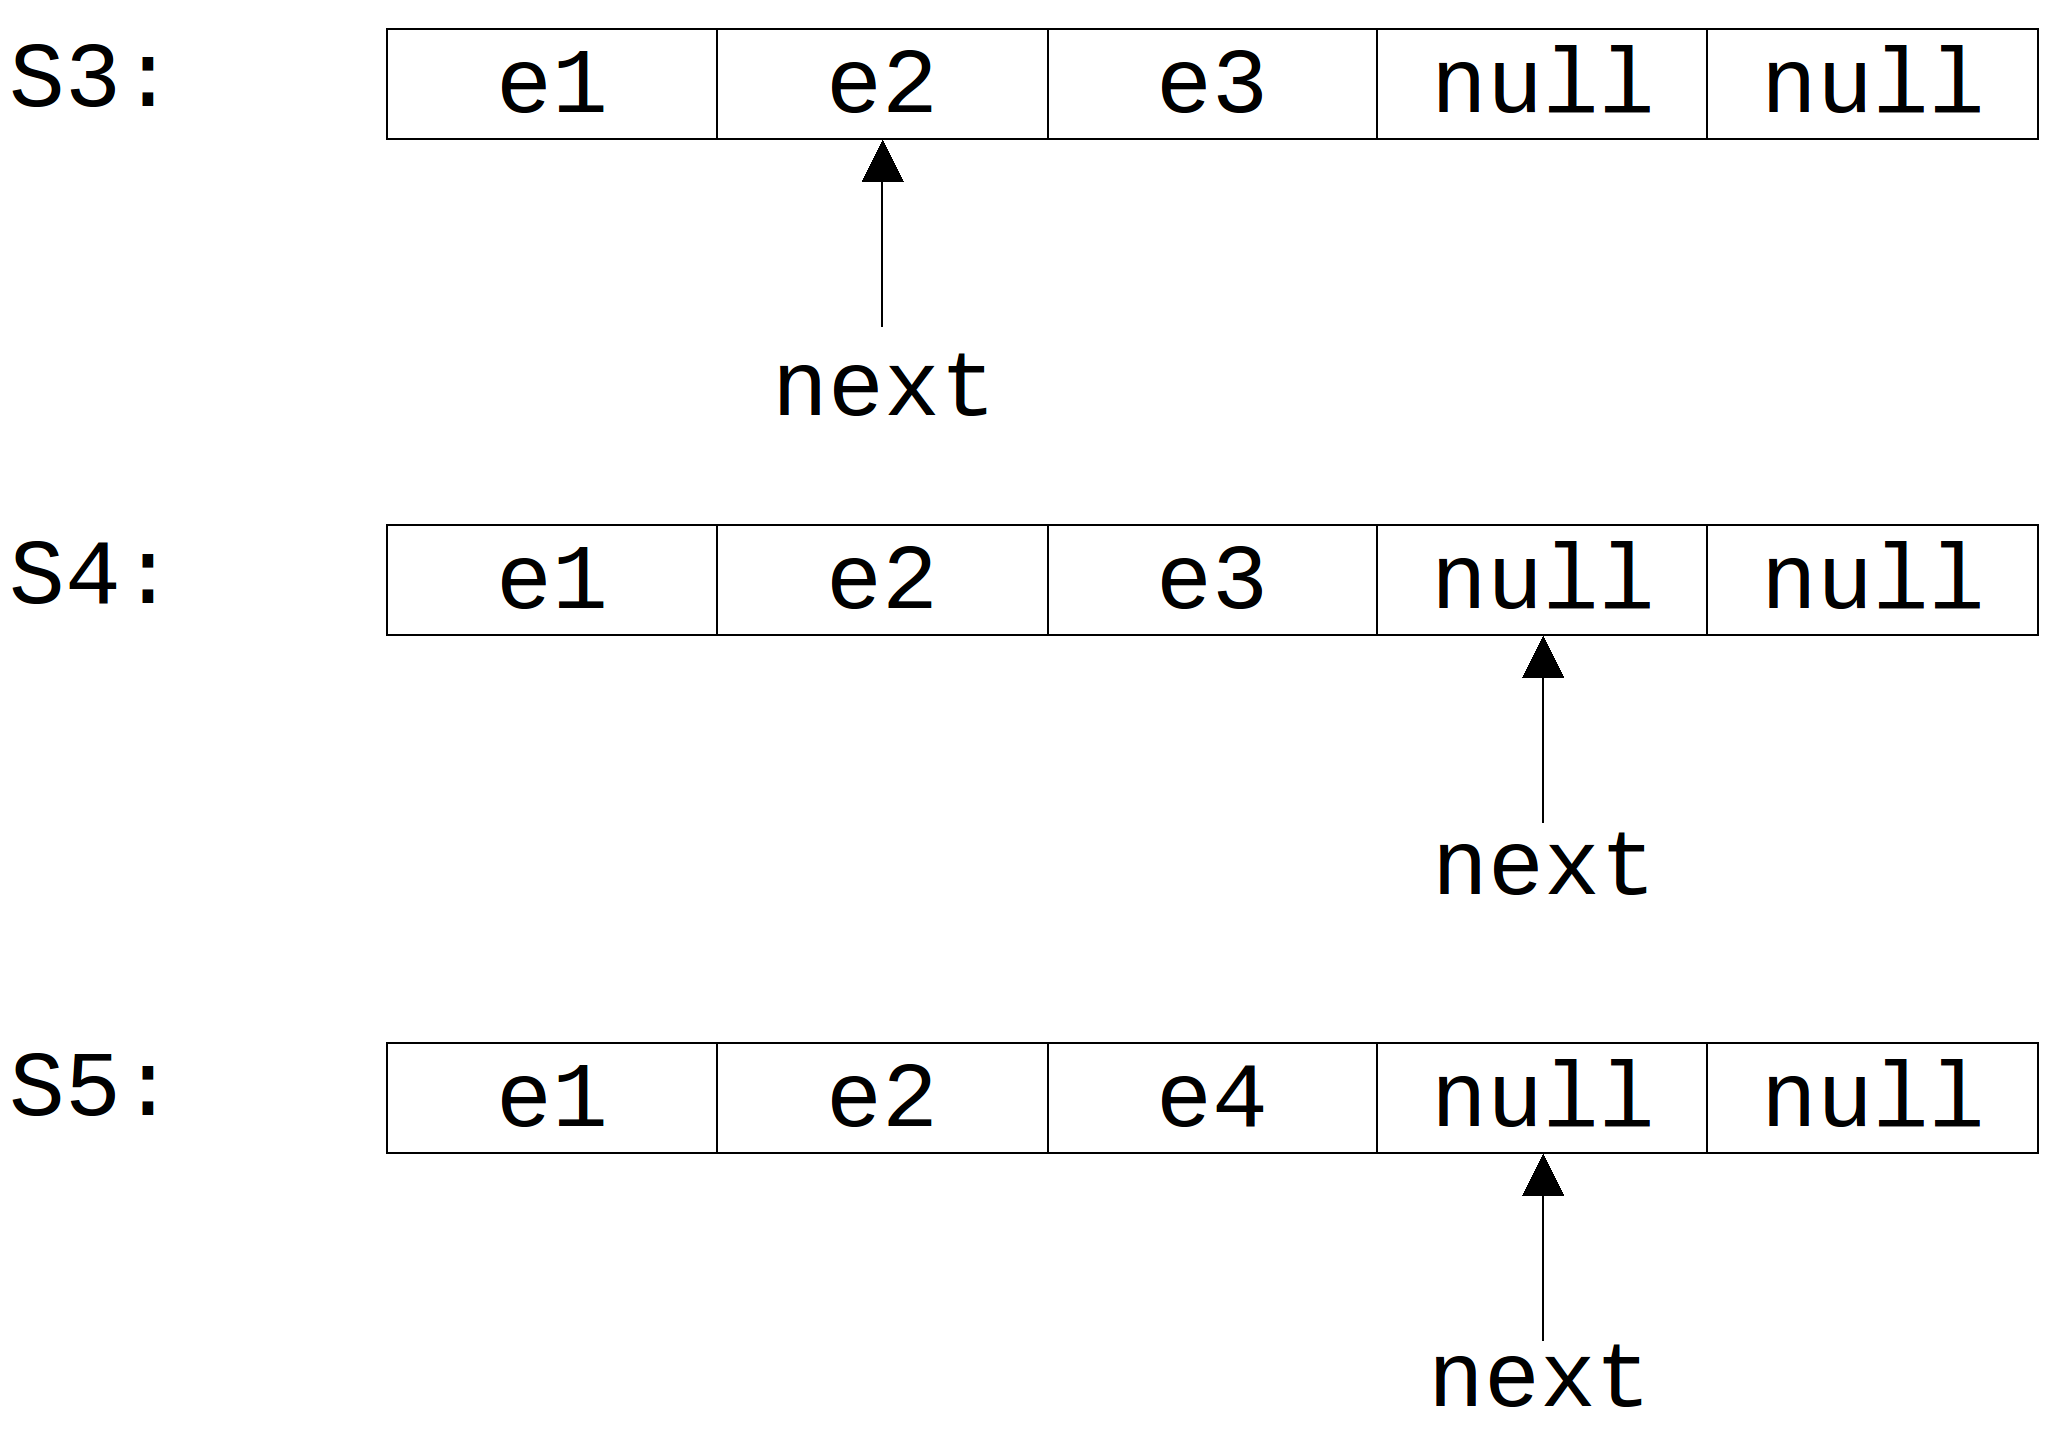
\includegraphics[scale=0.1]{img/undo_redo_cont.png}
\caption{ 復原及重做的運作(續) }
\label{fig:undo_redo_cont}
\end{figure}


承接圖~\ref{fig:undo_redo},當樂譜的狀態處於S2時,使用者可選擇繼續復原、重做或再執行一個新動作,如圖~\ref{fig:undo_redo_cont}。若繼續復原,樂譜會呼叫e2的revert(),左移next使樂譜進到S3。若重做,樂譜會呼叫e3的perform()並右移next,表示e3重回已執行的狀態,樂譜便進到S4。若執行新動作產生改動e4,樂譜則會先清空next及其右的所有改動(此時僅e3被移除),將e4填入next的位置再將next右移,代表e4已執行,而樂譜則進到S5的狀態。

我們用一個例子來解釋執行、復原、重做和訊息配發功能的運作過程。當使用者為樂譜新增一個聲部時,樂譜會將必要的資訊填入一個新產生的新增聲部改動(AddPartChange),「執行」該改動,然後將該改動儲存起來,再將其配發給所有已註冊的樂譜改動傾聽者,此時可能是一個負責繪製該樂譜的樂譜介面。而樂譜介面得知一個新增聲部改動發生後,便會重新繪製畫面。如此一來,使用者便可看到更新的樂譜。若使用者反悔想復原樂譜,樂譜也可對該改動執行「回復」,「回復」會再產生一個刪除聲部改動(RemovePartChange)。樂譜「執行」此刪除聲部改動以將剛產生的聲部移除,再以此改動通知該樂譜所有的樂譜改動傾聽者。由於此刪除聲部改動不是由使用者直接產生,故此改動不會被儲存起來。

\section{樂譜播放器}

樂譜播放器(撥放器,ScorePlayer)負責將樂譜撥放出來,讓使用者得以聆聽編輯中的樂譜。當使用者選擇「播放」後,播放器會先將編輯中的樂譜轉換為Sequence,再將該Sequence透過Sequencer播放出來。

/*********  移到 2.1 


\begin{figure}[htb]
\centering
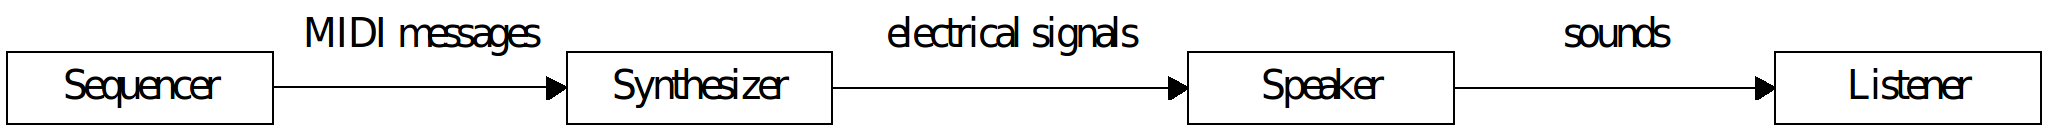
\includegraphics[scale=0.12]{img/play.png}
\caption{ Java Sound API中Sequence的播放流程 }
\label{fig:play}
\end{figure}


如圖 \ref{fig:play}所示,Sequencer在播放Sequence時,會將Sequence內的MIDI訊號依時間戳記依序送出,音源器(Synthesizer)根據接收到的MIDI訊號自音源庫中提取對應的電子訊號並送給喇叭(Speaker),喇叭則根據電子訊號產生聲音再由你我所接收。
移到 2.1    **********/ 


樂譜播放器也可讓使用者在執行期選擇音源器,例如在Windows作業系統下,除了Java平台內建的音源器Java Sound Synthesizer之外,使用者也可選擇系統內建的Microsoft MIDI Mapper和Microsoft GS Wavetable Synth兩種音源器。除了軟體音源器外,樂譜播放器也可將MIDI訊號送給外接的硬體音源器來產生聲音。不同的音源器會具有不同的音色,使用者可依其偏好自行選擇。 /* 內部如何與library 銜接 ?  */

我們以輸出裝置管理員(OutDeviceManager)來管理系統可使用的音源器。所有要撥放的MIDI訊號皆會送給輸出裝置管理員, 使用者可呼叫其setOutDevice() 方法選擇音源器。 /* 內部如何與library 銜接 ?  */

/*  漏解釋 樂譜播放器, 輸出裝置管理員 與 4.1 的關聯  */


\begin{figure}[htb]
\centering
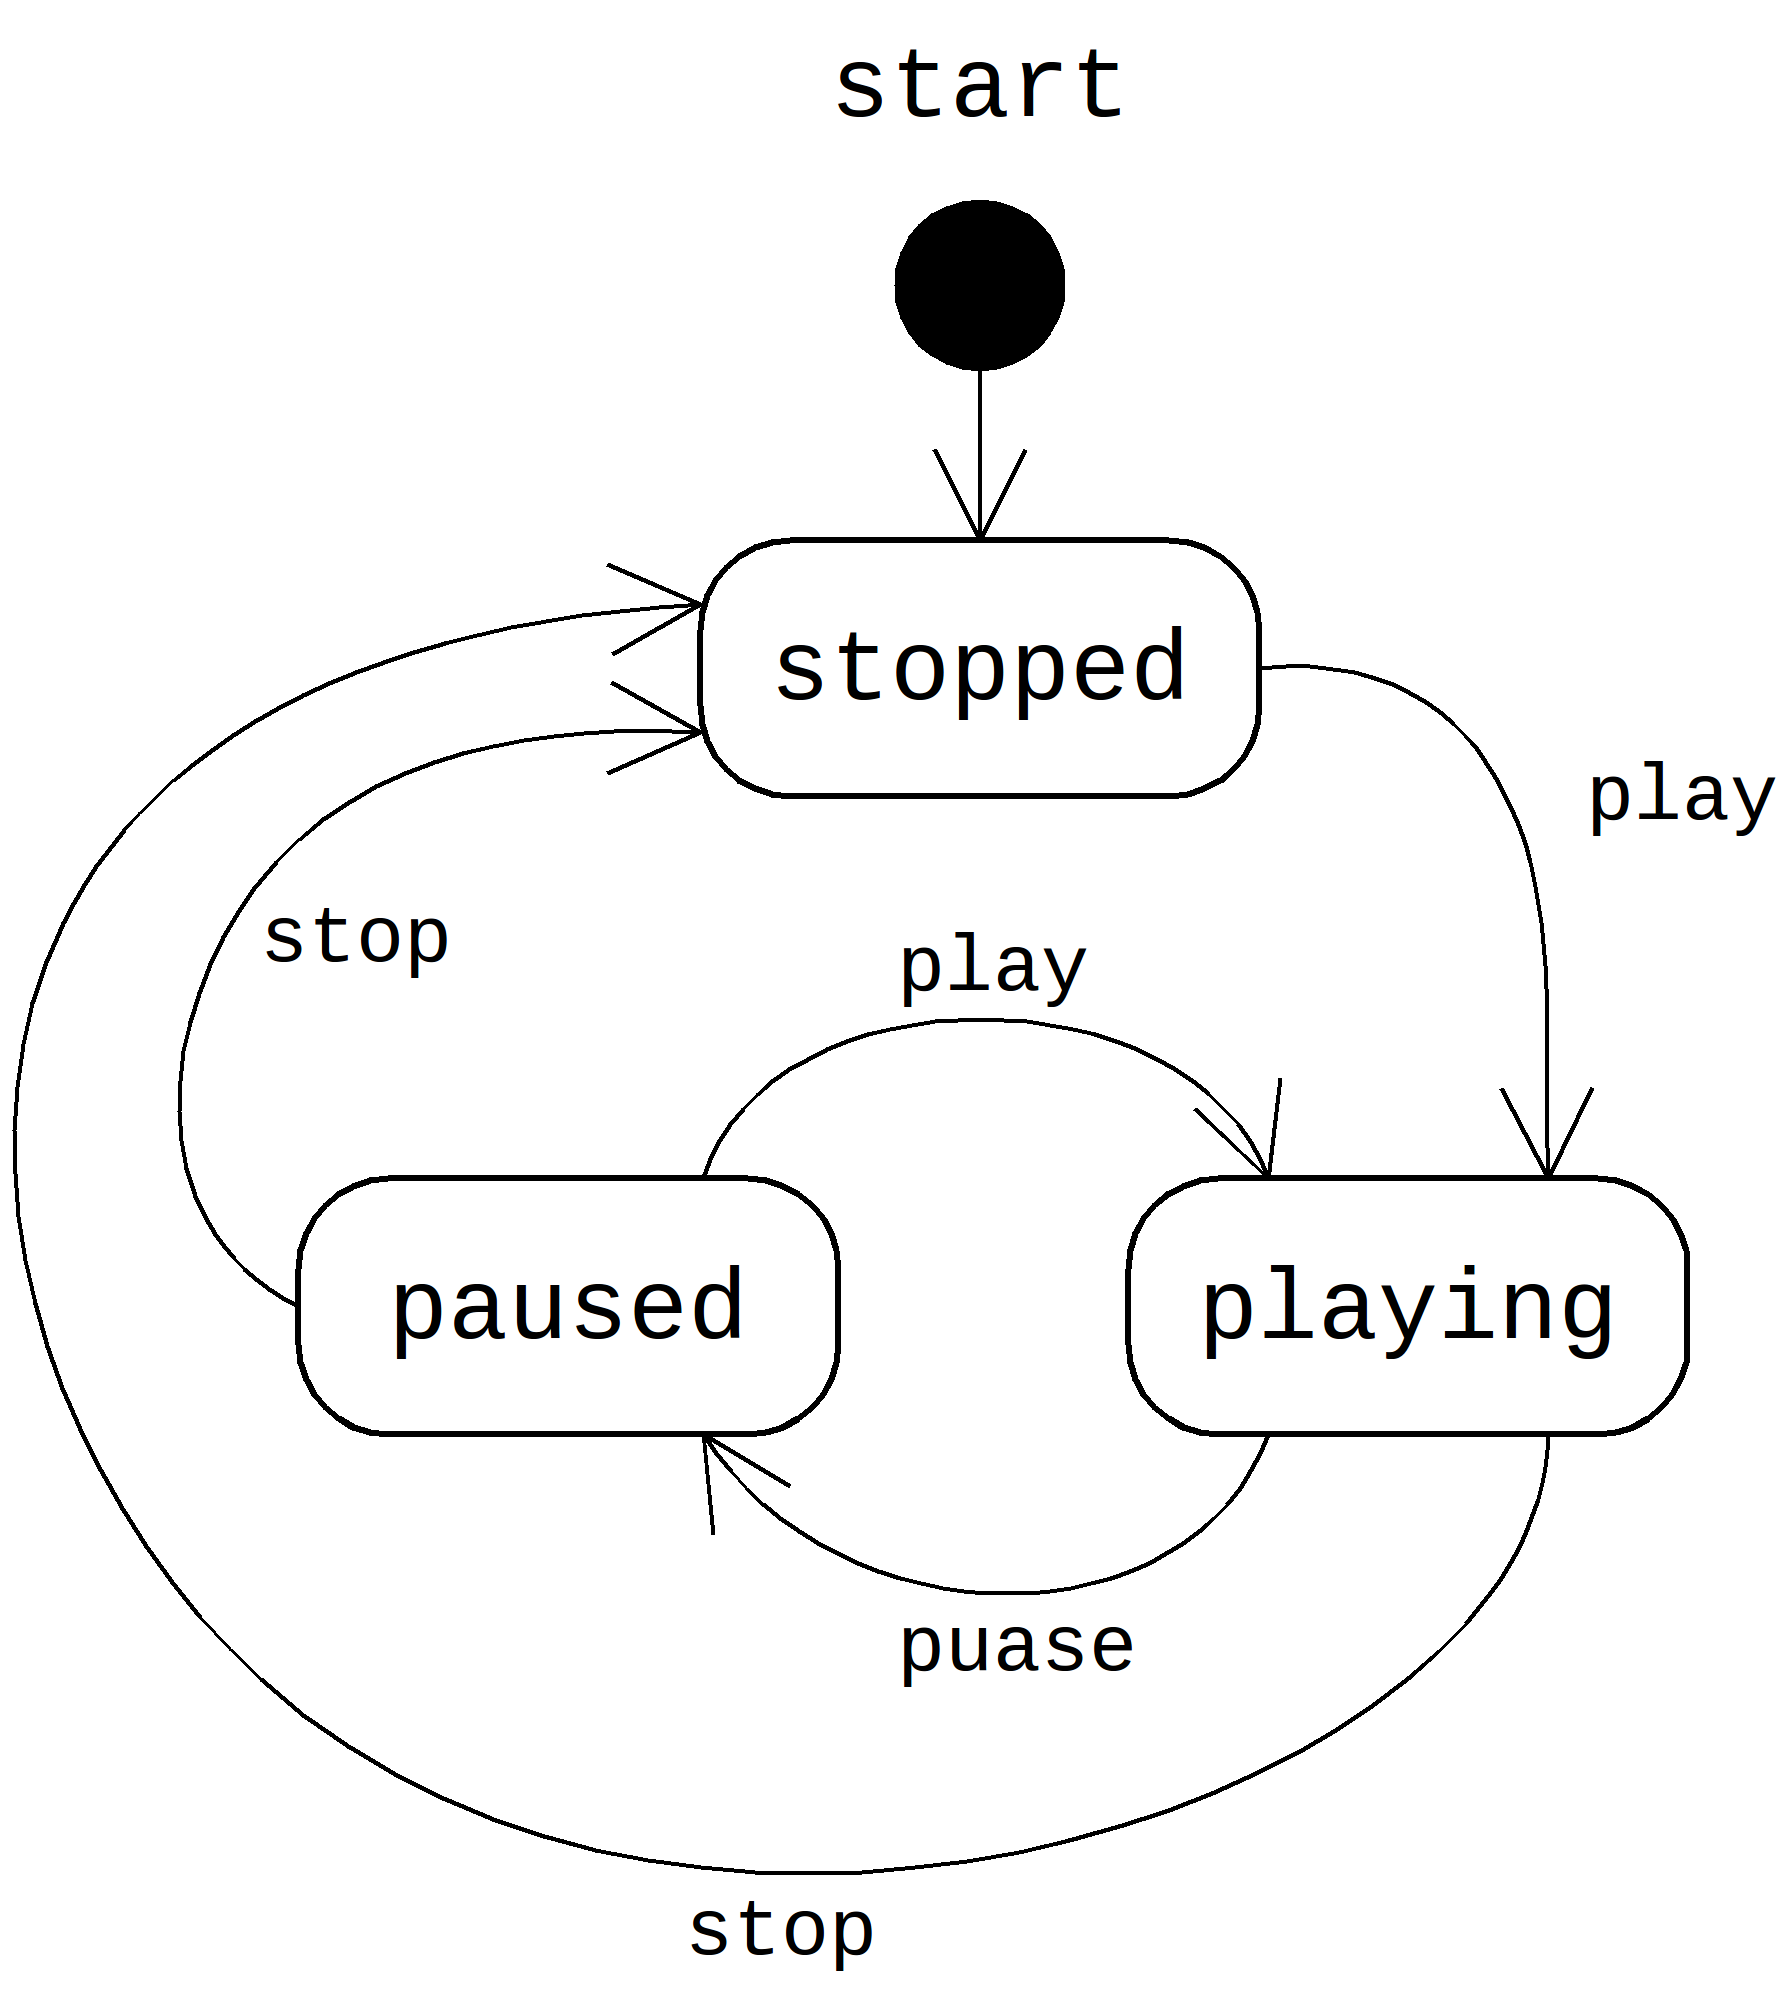
\includegraphics[scale=0.15]{img/player_states.png}
\caption{ 樂譜撥放器的狀態圖 }
\label{fig:player_states}
\end{figure}



/****** 移到CH3  
樂譜播放器具有三種不同的狀態,分別為停止狀態(stopped)、播放狀態(playing)及暫停狀態(paused)。在預設的情況下,播放器處於無聲的停止狀態。當使用者選擇「播放」後,播放器則會進到播放狀態並開始撥放樂曲,在播放狀態下,使用者可選擇「停止」回到停止狀態,或選擇「暫停」進到暫停狀態。在暫停狀態下,樂曲停止播放,若選擇「播放」可回到播放狀態,樂曲會從暫停的地方開始播放;若選擇「停止」,則讓播放器捨棄目前的撥放進度並回到停止狀態。
 移到CH3  ************/  


\section{腳本編輯器}

我們使用Java Scripting API來實作腳本編輯器。透過綁定功能將編輯器實體匯入腳本(script)的執行環境中,便可以腳本來控制編輯器實體的行為,並存取、修改其所包含的樂譜。
例如,若要為樂譜加上一百個C4音符,使用者可以撰寫如下的腳本。/* user怎麼操作? */

\begin{verbatim}
for(i=0; i<100; i++) { 
   dp.getScore().getParagraph(0).getPart(0).add(new Note(60));
}
\end{verbatim}

其中,dp即為編輯器的實體/* dp由何處取得? 還reserved word?  */,getScore()方法會傳回目前操作中的樂譜,getParagraph(0)會傳回該樂譜的第一節,getPart(0)則會傳回該節的第一個聲部,add(new Note(60))則對該聲部加上一個音高值為60的C4音符。而若想控制編輯器,例如執行復原動作,可以執行如下面的腳本。

\begin{verbatim}
dp.perform(dp.undoAction);
\end{verbatim}

腳本編輯器的預設語言為JavaScript,使用者也可自行安裝直譯器,便可以其他語言來控制編輯器和樂譜。

\section{立體聲編輯器}

在不受干擾的環境中,聽力正常的人們能輕易地辨認出聲源的位置。我們的大腦可依循多項線索來推知此資訊,如兩耳時間差(interaural time difference, ITD)及兩耳音量差(interaural level difference , ILD)。即便只剩單耳的聽力,人們也能單純透過音量(volume)和聲音通過頭部、肩膀及外耳造成的音量及音色變化來判斷聲源的位置,此變化可以頭部傳導函式(head-related transfer function, HRTF)[]來描述。

我們可以操縱這些線索來產生虛擬的音源。使用一般的雙聲道喇叭,透過改變兩喇叭放音的時間差或音量差便可讓大腦產生錯覺,讓人誤以為聲音是由不存在的音源所發出,便可用來模擬真實世界的聲音效果。這種方式所產生的聲音常稱為立體聲(stereophonic sound, stereo)。

Dolphin的立體聲編輯器則透過改變聲部的平衡(pan)和音量來決定樂器的位置。撥放時樂譜撥放器便會以音量和兩耳音量差來達到立體聲的效果。

立體聲編輯器以一虛擬的立體場域(stereo field)來讓使用者編輯立體聲效果,每個聲部的樂器會對應到立體場域上的一個虛擬聲源,如圖 \ref{fig:stereo_editor}。當虛擬聲源沿著立體場域的橫坐標移動便會改變虛擬聲源相對於聽者 /* 在哪裡?  */的方位,而當虛擬聲源沿著縱座標移動則會改變虛擬聲源相對於聽者的距離。  /* 如何使用? 應在CH3說明. */


\begin{figure}[htb]
\centering
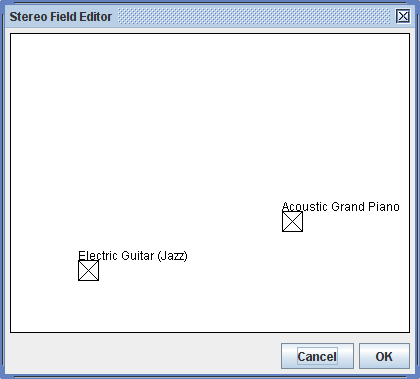
\includegraphics[scale=0.3]{img/stereo_editor.png}
\caption{ 立體聲編輯器的執行畫面 }
\label{fig:stereo_editor}
\end{figure}


虛擬聲源的方位決定於最外側的兩支喇叭和聽者連線的夾角,若夾角為180度,且虛擬聲源位於立體場域的最左方,則虛擬聲源會在聽者的正左方,播放時聲音便像由聽者的正左方傳來;而若夾角縮為90度,虛擬聲源會在聽者的左前方,而聲音便像由左前方傳來。  /*
理論沒講清楚!.
*/

聲音的音量和聲源至聽者的距離呈反比[21],當虛擬聲源為於立體場域的最下方時,我們定義虛擬聲源與聽者的距離為1,且其產生的音量為最大值;而當虛擬聲源為於立體場域的最上方時,定義虛擬聲源與聽者的距離為127。虛擬聲源的音量便是音量的最大值除以虛擬聲源與聽者的距離。 /*
實作沒講清楚: 左右聲道如何處理?
*/

\section{MIDI 檔的匯入與匯出}

Java Sound API 內的類別Sequence 用來表示樂曲,API 內建有讀取和寫出MIDI檔的方法。因此我們只需要實作Sequence 至Score的轉換,便可實作出MIDI 檔和樂譜的轉換。

/******  移置到4.8  
另外,為了使用Java Sound API提供的各項功能,我們實作了樂譜和Sequence的轉換函式。例如在播放樂譜時,我們先將樂譜「編譯」為Sequence,再利用Java Sound API播放出來;而在匯入MIDI檔時,則先使用Java Sound API讀進MIDI檔成為Sequence,再將其「反編譯」為樂譜,我們將在進一步解釋轉換的演算法。
移置到4.8  *******/

\subsection{匯入MIDI 檔}

和MIDI檔一樣,Sequence僅記錄音而不是音符。每個音以Note On訊息開始,以Note Off訊息(或強度為零的Note On訊息)結束。然而,Note On和Note Off僅含音高(pitch)和強度(velocity)兩樣和音符有關的資訊,並不包含時值。我們僅能由兩個MidiEvent中時間戳記的差來得到音的長度。然而一個音尚可能由多個以連結線(tie)連結的音符所產生,故我們以多次的解析過程來找出音符的個數及各音符正確的時值,Sequence 至Score的轉換可分為以下九個主要步驟: 

1. 讀入Sequence及各Track的基本屬性。 

Sequence的基本屬性會以MetaMessage紀錄在時間戳記為零的地方,此包含標題(訊息開頭為0x3)、預設的調號(訊息開頭為0x59)、拍號(訊息開頭為0x58)及節拍(訊息開頭為0x51)。Track的基本屬性則以ShortMessage紀錄在時間戳記為零的地方,包含樂器(訊息開頭為0xC0)、音量(訊息開頭為0xB7)及平衡(訊息開頭為0xBA)。我們建立樂譜、節及聲部並將對應的欄位填入其中。

2. 將NoteOn、NoteOff訊息轉換為音符(Note)。 

由Track的開頭開始掃描,遇到NoteOn(訊息開頭為0x90),便開始尋找對應的NoteOff(訊息開頭為0x80),或強度(Velocity)為零的NoteOn訊息(兩者皆可做為音的結束),找到後便依NoteOn訊息內的音高及兩則訊息時間戳記的差做為音長來建立音符。

3. 在音符間插入休止符。 

第二個步驟僅建立有聲音符,音符間尚可能含有停頓,我們從頭掃描第二個步驟所建立的音符,並在停頓處建立休止符。休止符的長度則為前一個有聲音符的結束至後一個有聲音符的開頭的差。

4. 將互為和弦的音符串接起來。 

此時有聲音符間可能彼此重疊,故重頭掃描有聲音符,將彼此重疊的音符串接為和弦音符。

5. 將過長的音符拆開。 

目前所建立的音符時值皆未經過驗證。重頭掃描音符,先將超過全音符時值的音符拆開為較短音符的集合,並以連接線連結。

6. 將橫跨小節線的音符拆開。

橫跨小節線的音符會造成錯誤的小節長度,故必須將其拆解。我們從頭掃描音符,並累計音符時值,若累計時值超過小節長度,便將最後掃描的音符拆為兩個音符,第一個音符填滿小節長度,剩餘的時值則納入第二個音符,再將兩個音符以連接線連結。

7. 尋找並建立三連音。 

嘗試以三連音解析剩餘的不合法音符。從頭掃描不合法音符,若其時值符合三連音的時值,便將其設為三連音。

8. 尋找並建立附點音符。

附點和連結線皆可延長音符的長度,但除了休止符外,附點音符皆可以連結線表示[],為免轉出的樂譜不含附點,故先解析附點音符。從頭掃描不合法音符,將含有附點的音符建立附點。

9. 拆解剩餘的不合法音符。

將剩餘的不合法音符拆解為合法音符的集合,並以連接線連結。

\subsection{匯出MIDI 檔}

如同匯入MIDI 檔的演算法,我們只需要實作Score 至Sequence 的轉換,便可匯出MIDI 檔:

1. 根據MIDI規格寫出樂譜及各聲部的基本屬性,包含樂譜名、拍號、調號、速度、音量,及平衡。 

2. 將音符(Note)轉換為NoteOn及NoteOff訊息。 

由各聲部開頭開始寫出音符,將每個音符寫為對應的NoteOn和NoteOff訊息。

3. 為音符加上節奏資訊

以強度值100(最高為127)為強拍,80為弱拍設定音符的節奏資訊。二拍為強、弱,三拍為強、弱、弱,四拍為強、弱、強、弱,五拍為強、弱、強、弱、弱,六拍為強、弱、弱、強、弱、弱,並為每小節的第一拍增加強度值10。



\chapter{結論與展望}

Dolphin除了有基本的樂譜編修能力,也具備許多其它同類型軟體普遍缺乏的自動化功能,如立體聲編輯器、哼唱輸入、五線譜與簡譜的即時轉換、MIDI檔與樂譜的轉換,以及腳本編輯器。

然而Dolphin仍有許多待改進之處,如加強哼唱輸入的效能和準確性、改善MIDI轉譜的正確性、擴充音樂符號、歌詞輸入及列印等,我們希望能繼續開發使其更為完善。

Dolphin 為一開放源碼的自由軟體,以GPL 釋出。


\appendix

\chapter{哼唱輸入}

Dolphin的哼唱輸入能將使用者對麥克風的哼唱轉換成對應的音符並立即在螢幕上顯示出來,其功能類似於語音輸入(speech-to-text)。但在輸入上,語音輸入使用的是各種語言的口語(spoken language),而哼唱輸入則是接收使用者的哼唱,使用者可發出各種聲音,而不限於哼音名或唱名。在輸出上,語音輸入的輸出是文字,而哼唱輸入的輸出則是音符。而在操作方式上,一般語音輸入採逐字輸入,而哼唱輸入則模仿語音輸入,採「逐音輸入」的方式來輸入音符。當使用者哼出一個音,系統便即時地產生出一個音符。哼唱輸入也可視為以人聲為輸入的「自動旋律轉錄」(automatic melody transcription)。

要由哼唱得出旋律,我們必須先將哼唱的音與音分離出來。我們採用簡單的端點偵測(End-Point Detection)[]技巧,以「停頓」來做為音與音的分離標記。哼唱輸入啟動後便會開始擷取(capture)聲音,若發現聲音的強度(intensity)大於某臨界點,便開始錄製(record),而若聲音的強度低於該臨界點,代表已經過一定的停頓,便停止錄製;每次錄到的聲音樣本便視為一個音。此法要求使用者在哼唱的音與音間留有一定的停頓以切出正確的音。

分隔音與音後,我們再求每個音的時值和音高。時值可由樣本的長度求得。樣本的開始至結束所經過的時間再搭配節奏的資訊便可決定音符的時值。

我們利用JPraat的音高追蹤演算法實作從樣本計算出連續的基本頻率,再根據MIDI Tuning Standard[]將其平均帶入下式以將基本頻率映射至MIDI的音高值(pitch number):

%p=69+12*log2(f/440)
\[
p=69+12\times\log_2{\left(\frac{f}{440}\right)}
\]

其中,\(p\)代表音高值,\(f\)為基本頻率(單位為Hz)。計算出音高及音長兩項資訊後,系統便可產生出對應的音符。再利用傾聽者的機制將音符填入樂譜介面的游標位置,便可完成哼唱輸入。

然而,每個人的音域都不盡相同,當人哼出旋律時,往往唱不出所想的音高。為此,我們以事先校準的方式來得到補償值,在實際哼唱時系統便可依該值自動補償哼唱者的音高。
\chapter{Praat及音高追蹤}

Praat是一套由阿姆斯特丹大學的Paul Boersma和David Weenink所開發的開放原始碼語音分析軟體。

Praat可將聲音樣本利用快速傅立葉轉換(fast Fourier transform, FFT)轉換為頻譜圖(spectrogram)。頻譜圖通常以彩色的二維圖表示,圖 \ref{fig:spectrogram}即為一女聲的頻譜圖,其中橫座標為時間,縱座標為頻率,而顏色則代表強度。

\begin{figure}[htb]
\centering
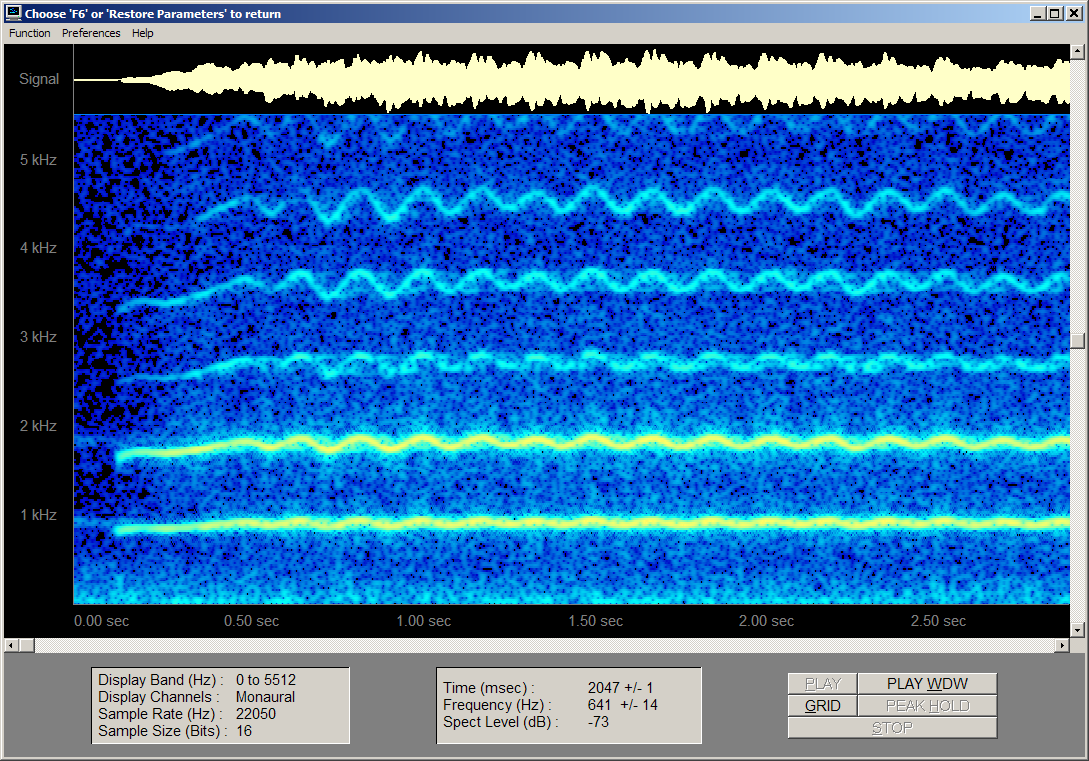
\includegraphics[scale=0.3]{img/spectrogram.png}
\caption{ 一段女聲的頻譜圖 }
\label{fig:spectrogram}
\end{figure}

自然界或樂器所發出的聲音通常由許多頻率不同的純音(pure tone)所組成,其中頻率最低的音稱為基音(fundamental tone),其餘的音稱為泛音(overtone),基本頻率(基頻,fundamental frequency)即為基音的頻率。

人對聲音基本頻率的感受即為音高(pitch)。高基頻造成高音高,低基頻造成低音高。例如敲擊音叉所產生聲音的基本頻率約為440 Hz,相當於鋼琴中間La(A4) 的音高。

Praat可由頻譜圖進一步計算出聲音的基本頻率。在音訊處理領域,此技術稱為音高追蹤(pitch tracking)。圖 \ref{fig:pitch_tracking}為Praat 對鋼琴彈奏出的C Major Scale 執行音高追蹤的結果。


\begin{figure}[htb]
\centering
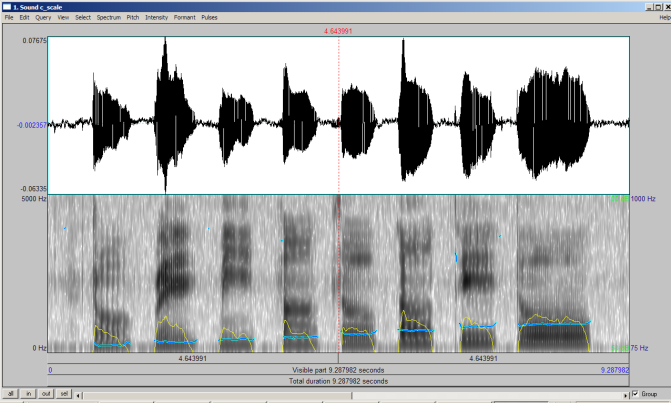
\includegraphics[scale=1.0]{img/pitch_tracking.png}
\caption{ Praat的音高追縱。上方為輸入聲音樣本的波型圖,下方為該樣本的頻譜圖及音高追縱後的結果。 }
\label{fig:pitch_tracking}
\end{figure}


為了使用Praat[]的音高追蹤演算法實作來判斷音高。我們翻譯了約三千行Praat的C 程式碼成為一套Java 程式庫JPraat,內含有計算聲音強度,音高追蹤及快速傅立葉轉換的實作。

% bibliography
\begin{thebibliography}{99} % the arg is for the width of the item label
\bibitem{wiki}
  \url{http://en.wikipedia.org/wiki/Gongche_notation}
\bibitem{britannica}
  \emph{Encyclopædia Britannica}, vol. 24, p. 536
\bibitem{designPattern}
  Gamma, R Helm, R Johnson, J Vlissides, 
  \emph{Design Patterns: Elements of Reusable Object-Oriented Software},
  Addison-Wesley, p. 163, 293, 
  1994
\bibitem{chinaMusicHistory}
  薛宗明《中國音樂史.樂譜篇》, p. 549
\bibitem{chinaEncyclopedia}
  《中國大百科全書.音樂舞蹈》, p. 299
\end{thebibliography}

% 參考文獻   /* 沒有書才用網頁 */
% 1. 清蔚科技,「哼唱鈴i-Ring」,http://www.cweb.com.tw/About/AboutIndex.hi,2009。
% 2. Aspire Software, “Music MasterWorks,” http://www.musicmasterworks.com/, 2009.
% 3. Avid Technology, “Sibelius 5,” http://www.sibelius.com/, 2009.
% 4. “Denemo 0.82”, http://www.denemo.org/, 2009.
% 5. E Gamma, R Helm, R Johnson, J Vlissides, “Design Patterns: Elements of Reusable Object-Oriented Software,” Addison-Wesley, p. 163, p. 293, 1994
% 6. End Point Detection, http://neural.cs.nthu.edu.tw/jang/books/audioSignalProcessing/epdIntro.asp?title=6-1%20Introduction%20to%20End-Point%20Detection%20(%BA%DD%C2I%B0%BB%B4%FA%A4%B6%B2%D0)
% 7. Eric Taylor, “The AB Guide to Music Theory Part I,” The Associated Board of the Royal Schools of Music, p. 17, 1989. 
% 8. Sound Pressure, http://en.wikipedia.org/wiki/Sound_pressure, 2009
% 9. Tracy V. Wilson, “How Virtual Surround Sound Works” http://electronics.howstuffworks.com/virtual-surround-sound.htm/printable, 2009
% 10. “LilyPond”, http://lilypond.org/, 2009.
% 11. MakeMusic, “Finale 2009,” http://www.finalemusic.com/, 2009.
% 12. MIDI Tuning Standard (MTS)>>>>>>>>>>>>>>>>>>
% 13. Paul Boersma & David WeeninkPraat, “Praat,” http://www.praat.org/,2009.
% 14. Piano Roll, http://en.wikipedia.org/wiki/Piano_roll
% 15. Sun Microsystems, “Java Sound API,” http://java.sun.com/products/java-media/sound/, 2009.
% 16. Sun Microsystems, “Java Platform, Standard Edition,” http://java.sun.com/javase/index.jsp, 2009
% 17. Sun Microsystems, “Java Scripting API,” https://scripting.dev.java.net/, 2009.
% 18. “Vocal Range,” http://en.wikipedia.org/wiki/Vocal_range, 2009.


\end{document}


